This problem will analyze the following unity gain feedback control system:
\begin{center}
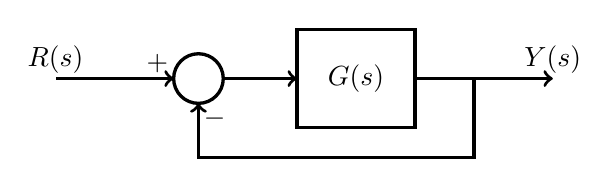
\begin{tikzpicture}[scale=1,inner sep=0pt,outer sep=0pt,very thick,
sysblock/.style={draw,rectangle,inner sep=2pt,minimum width=1.5cm,minimum height=1.25cm,very thick}]
\draw (5,0) node[draw,circle] (sum3) {$\rule{0pt}{18pt}$};
%\draw (7,0) node[draw,circle] (sum2) {$\rule{0pt}{18pt}$};
\draw (7,0) node[sysblock] (G) {$G(s)$};

\draw[<-] (sum3.180)  node[above left=2pt] {$+$} -- ++(-1.5,0) node[above=2pt] {$R(s)$};
\draw[->] (sum3.0) -- (G);
\draw[->] (G) -- ++(2.5,0) node[above=2pt] {$Y(s)$};
\draw[->] (G) ++(1.5,0) -- ++(0,-1)  -| (sum3.-90) node[below right=2pt] {$-$};
\end{tikzpicture}
\end{center}
$G(s)$ is stable. The Bode plot of $G(s)$ is shown below. 
\begin{center}
\includegraphics[width=5.5in]{\mainfolder/LectureNotes/\lecturefolder/HomeworkProblems/Problem03/prob3}
\end{center}
Sketch the Nyquist plot, and determine if the closed loop system is stable.
